La schermata "\textit{Calibration}" è usata per calibrare l'applicazione e apprendere lo spazio di movimento massimo dall'occhio.

Come è mostrato in figura \ref{fig:calibration} sullo schermo sono mostrati dei punti che alternativamente lampeggiano, l'utente è cosi portato a guardare il punto lampeggiante.

In questo modo è stato possibile apprendere lo spazio di movimento dell'occhio sullo schermo.

\begin{figure}[htbp]
    \centering
    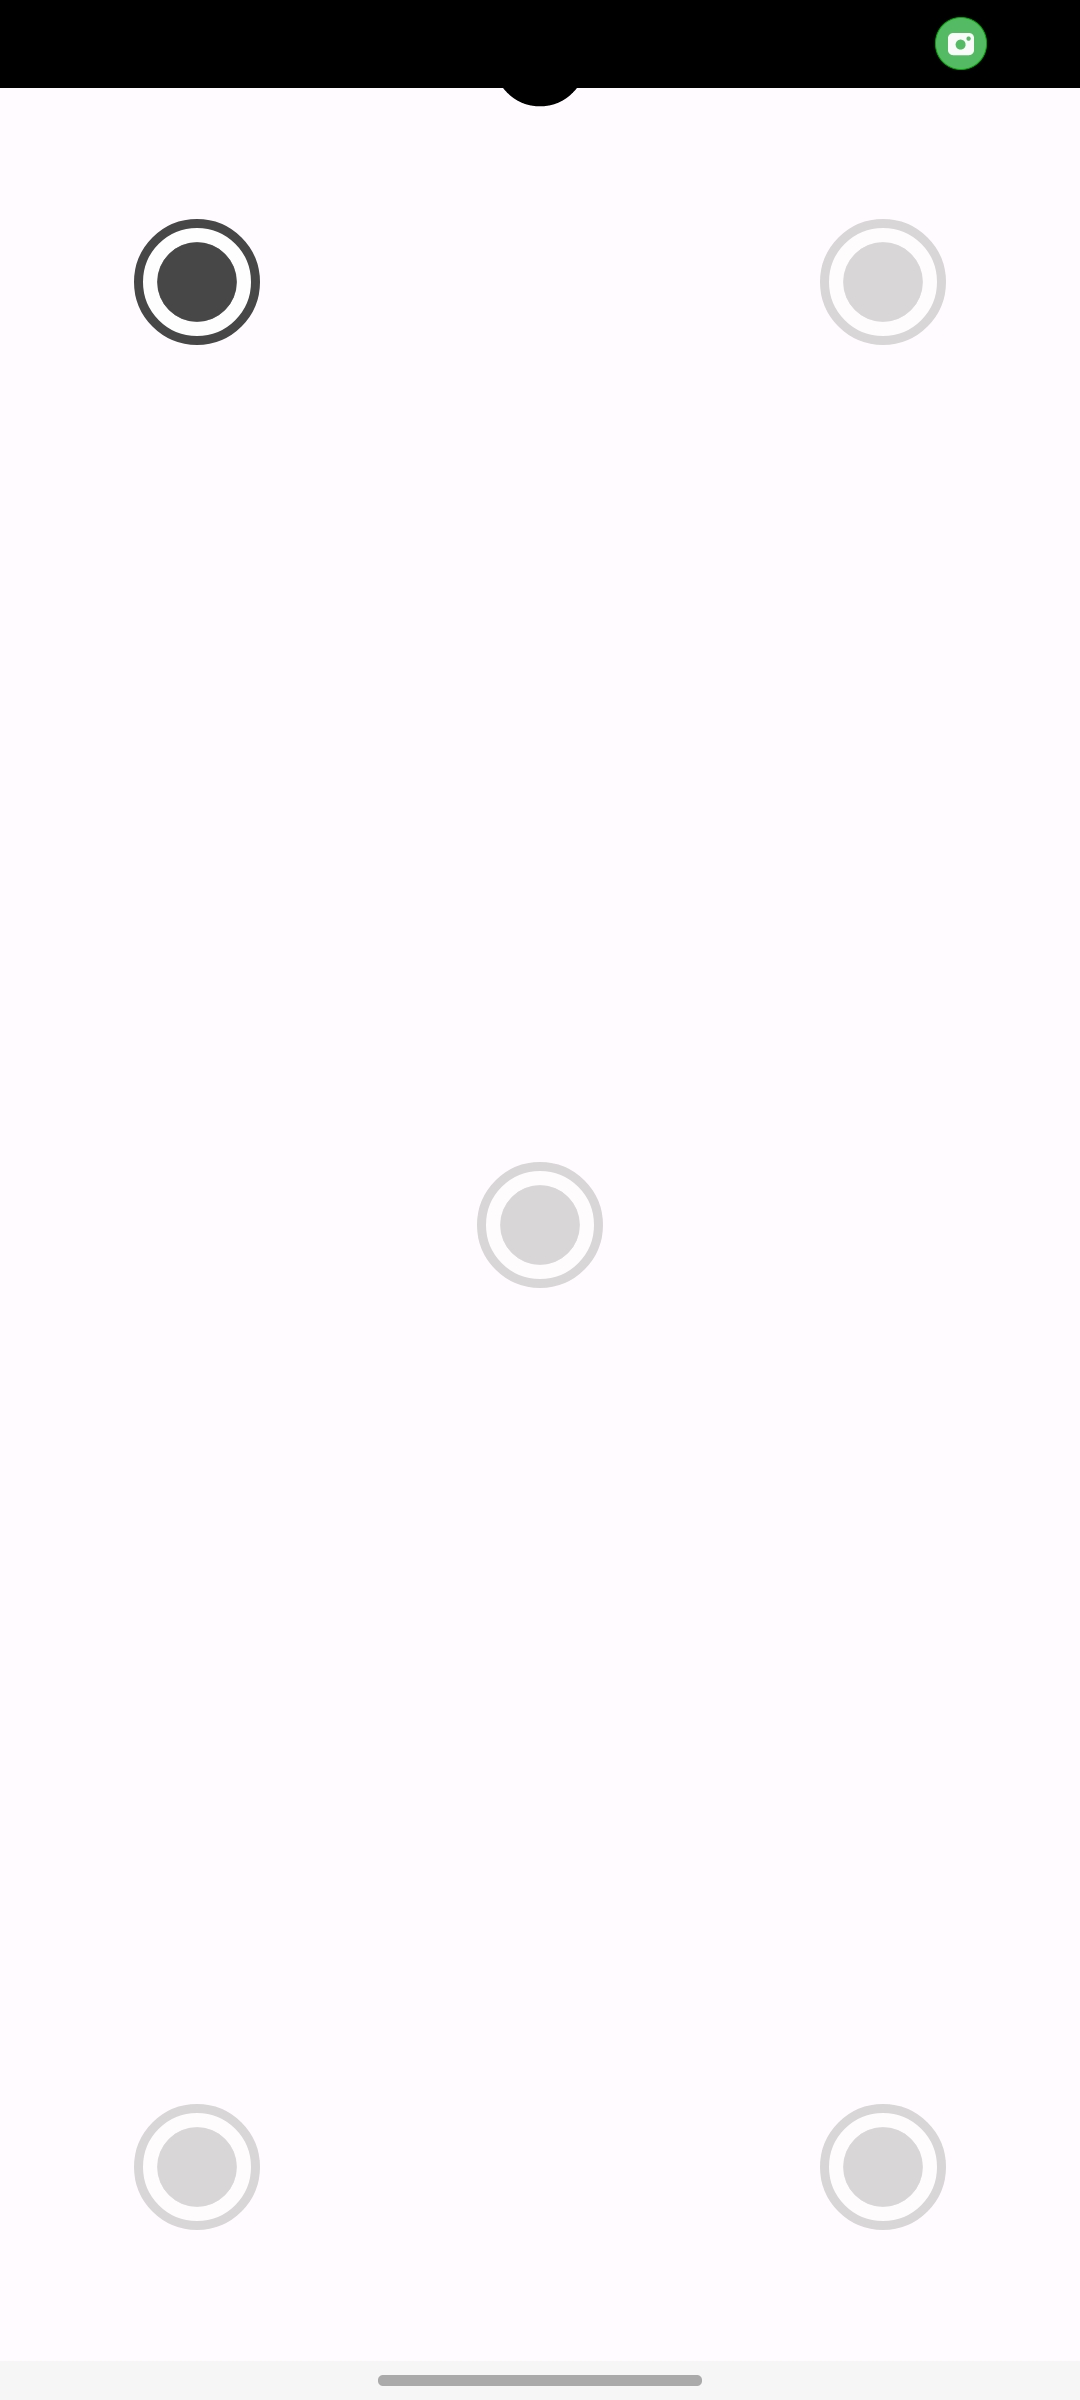
\includegraphics[scale=0.12]{ProgettoAndroid/Calibration/Images/CameraApp_Screen_calibration.jpg}
    \caption{Schermata Calibration}
    \label{fig:calibration}
\end{figure}